\chapter{Quantum Machine Learning}

\epigraph{Would I rather be feared or loved? Easy. Both. I want people to be afraid of how much they love 
me.}{Michael Scott}

A new interdisciplinary research topic that goes by the name of Quantum Machine Learning
(QML) has recently begun to explore the interplay of ideas from quantum computing and
machine learning [1].
For example, QML investigates whether quantum computers can speed up the time it takes
to train or evaluate a machine learning model. On the other hand, the QML community
leverages techniques from machine learning to devise new quantum error-correcting codes
[2], estimate the properties of quantum systems, or develop new quantum algorithms.
The investigations of Machine Learning and Quantum Computation can be factorised in four main areas (as shown in
figure):


\begin{itemize}
    \item \textbf{Classical for Classical (CC)}.\\ This area actually do not have a quantum component and 
    it indicates those purely classical cases when a classical machine learning algorithm is used to solve 
    a classical task.
    \item \textbf{Classical for Quantum (CQ)}.\\ This area indicates those studies which aim to use classical
    machine learning procedures to deal with problems in the quantum physics domain.
    \item \textbf{Quantum for Classical (QC)}.\\ This area instead refers to using quantum resources or algorithms, 
    for example variational quantum algorithms, to analyse or process classical information, 
    that is data that come from a classical source.
    \item \textbf{Quantum for Quantum (QQ)}.\\ This last area is arguably the most compelling yet unexplored
    application of Quantum Machine Learning, regarding the use of quantum processors to
    learn or study properties of quantum systems.
\end{itemize}


\section{Variational Quantum Algorithms}

Variational Quantum Algorithms (VQAs) are the leading proposal to exploit current quantum computing platforms, 
based on the hope that it is possible to achieve a meaningful quantum advantage already in the non error-corrected 
regime, before standard quantum algorithms, like Shor’s factoring, can be realised at scale. 
Therefore, since NISQ devices are limited in size and inherently noisy, VQAs circumvent the problem simply by using 
them as little as possible, only for the bare minimum, while outsourcing all remaining tasks to a classical computer.
This approach leads to an hybrid paradigm in which quantum and classical computational resources are used in combination 
to solve a task.
Moreover, Variational Quantum Algorithms can be seen as the quantum counterparts of highly successful machine 
learning methods, such as neural networks. 
Because of the challenges posed by NISQ devices, VQAs employ \textit{parameterized 
quantum circuits} that can be feasibly executed on current quantum computers. The optimization of these parameters, 
achieved through minimizing a \textit{cost function}, is usually delegated to a classical optimizer, making use of the 
classical computer's capabilities.
Therefore, the trademark of VQAs is that they use a quantum computer to estimate the cost function (or its gradient) 
while leveraging the power of classical optimizers to train the parameters.

\subsection{Cost Function}

Variational Quantum Algorithms encode the solution of a task in the minimum of a cost function $C(\boldsymbol{\theta})$,
which depends on the parameters $\boldsymbol{\theta} \in \mathds{R}^n$ of the parameterized quantum circuit $U(\boldsymbol{\theta})$ contained in the algorithm.
Therefore the ultimate goal of these algorithms is to find the optimal set of parameters, which minimizes the
cost function:

\begin{equation}
    \theta_{opt} = \operatorname{arg\,min}_{\theta} C(\theta)
\end{equation}

A cost function is a scalar function $C(\boldsymbol{\theta}) : \mathds{R}^n \rightarrow \mathds{R}$, 
which could be often expressed as:

\begin{equation}
    C(\boldsymbol{\theta}) = \sum_{k} f_k(Tr(O_k \rho_{\theta}))
\end{equation}






\subsection{Parametrized Quantum Circuit}

VQAs are learning-based procedures that tackle a problem by encoding its solution in the 
minimum of a \textit{cost function} C(\textbf{$\theta$}) depending on some tunable parameters \textbf{$\theta$}, which
are part of the Ansatz




\section{Classical Machine Learning}

The term \textit{Machine Learning} was coined in 1959 by Arthur Samuel, an IBM employee and pioneer 
in the field of computer gaming and artificial intelligence.
The term \textit{Machine Learning} is often interchanged with other terms, such as \textit{Deep Learning}, 
\textit{Artificial Intellingence} (AI) and \textit{Artificial Neural Networks} (ANN) but they have different 
meanings.
AI \textit{is the science and engineering of making intelligent machines} (John McCarthy ‘56). 
AI has many branches: \textit{Machine Learning}, \textit{Deep Learning} and \textit{Artificial Neural Networks} 
are three of them.
Actually the hierachy is a little more complex: \textit{Artificial Neural Networks} is a sub-field of 
\textit{Deep Learning}, which is a sub-field of \textit{Machine Learning}.\\

\begin{figure}[h]
\centering
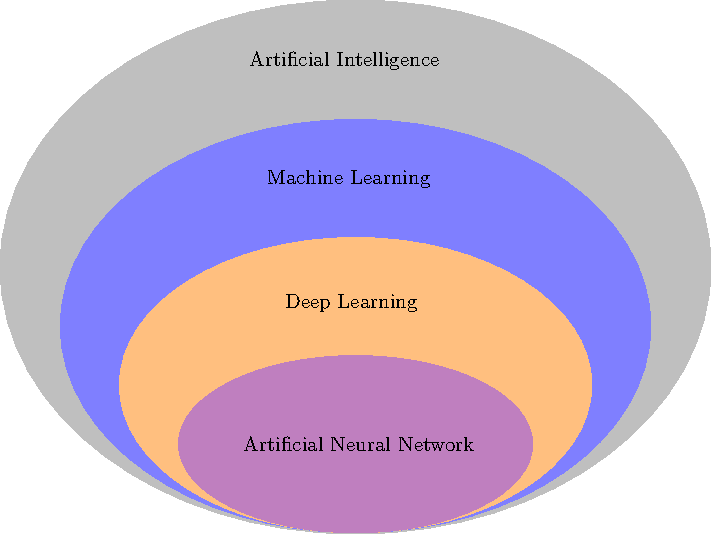
\includegraphics[scale=0.8]{Chapters/Chapter3/Images/venn.pdf}
\caption{Venn diagram representing the relationship between AI, Machine Learning, Deep Learning and ANN.}
\end{figure}

The term \textit{Machine Learning} refers to more than 60 different algorithms and they can be divided 
into three main paradigms, \textit{supervised}, \textit{unsupervised} and
\textit{reinforcement learning}, depending on how the algorithm interacts with the data to be analysed, and
the corresponding task to be solved. These can be summarised as follows:

\begin{enumerate}

\item \textbf{Supervised learning}: the algorithm is asked to reproduce the mapping between a set of
inputs and desired outputs, and then extrapolate the acquired knowledge also on other data
that was not used during training. In this case, the dataset provided to the algorithms consists
of a pair of numbers, the input to be processed, and the correct result that the machine
should output. The term “supervised" conveys the fact that, while training, the algorithm has
a target output that it has to reproduce.
\item \textbf{Unsupervised learning}: the algorithm has only access to inputs, without any informations
on the desired outputs. 
The main purpose of these algorithms is to identify patterns in the data.
The term “unsupervised" indicates that the algorithm do not require any human supervision or suggestion 
(such as the correct result) to function.
\item \textbf{Reinforcement Learning}: the algorithm has no dataset to process, rather it gets \textit{generated}
by the algorithm itself while running, specifically by the interaction between the \textbf{agent} and the 
\textbf{environment}.
Indeed, in the reinforcement learning framework, the algorithm, also referred to as an \textbf{agent}, 
interacts with an \textbf{environment} by performing \textbf{actions}.

\end{enumerate}

While these three paradigms indicates the historical classification of machine learning algorithms, many new
approaches are emerging, such as: semi-supervised learning, selfsupervised learning, continual learning and 
transfer learning.

In the following sections, the basic definitions and tools of machine learning will be discussed, particularly in
the context of supervised learning, which is not only the most common and easiest way to introduce
machine learning concepts, but is also the learning scenario used for the quantum machine learning
models discussed in this work.

\section{Quantum Machine Learning}

\subsection{Linear quantum models: quantum classifiers and kernel methods}

\subsection{Data reuploading models and Quantum Neural Network}

\subsection{Deriving the Fourier expansion}

\subsection{A single-qubit data reuploading circuit}

\subsection{Quantum Neural Networks}

\subsection{Generalization of QML models}

\subsection{The power of quantum machine learning}







